\chapter{Technical Architecture}
\label{ch:arch}

This chapter specifies the complete forecasting system: the winding-flux data
and how it is represented (\S\ref{sec:data}), the Convolutional LSTM cell and the
encoder--forecaster assembled from it (\S\ref{sec:convlstm}--\S\ref{sec:model}),
and the training procedure (\S\ref{sec:training}). Every design choice that
affects the reported results---in particular the spatial low-pass and the choice
of the \emph{accumulated} winding field---is stated explicitly so that the
outcome in Chapter~\ref{ch:results} can be read without hidden assumptions.

\section{Data and representation}
\label{sec:data}

\paragraph{Winding-flux datacubes.}
The input data are per-active-region datacubes derived from SDO/HMI
observations. Each cube stores a single channel $\mathrm{wind}[H,W,T]$---the
winding-flux density on an $H\times W$ spatial grid at $T$ successive times---
together with a vector of acquisition timestamps at a nominal $12$-minute
cadence. A small number of frames are missing; these are flagged by a sentinel
timestamp of zero and are removed before any windowing, so that the model only
ever sees physically contiguous sequences. The corpus used here comprises the
available HARP cubes; one cube exhibiting pathological, noise-dominated values
is excluded from every experiment.

\paragraph{The signed field and its dynamic range.}
Winding-flux density is a \emph{signed} pseudoscalar with a very large dynamic
range: physical magnitudes span several orders of magnitude, and a few
pathological pixels can reach far beyond the bulk of the distribution. Training
on such raw values is unstable. The field is therefore passed through a
sign-preserving \emph{inverse hyperbolic sine} (asinh) transform,
\begin{equation}
  \tilde{w} \;=\; \operatorname{asinh}\!\left(\frac{w}{s}\right),
  \qquad s = 10^{3},
  \label{eq:asinh}
\end{equation}
which is linear for $|w|\ll s$ and logarithmic for $|w|\gg s$. This compresses
the extreme tail while preserving sign and small-signal structure; the softening
constant $s=10^{3}$ was fixed by prior probing of the field's amplitude
distribution. The transformed field is then rescaled by a robust ($99.5$th
percentile) amplitude and clipped to $[-1,1]$ per cube, giving a normalised,
zero-centred representation comparable across active regions.

\paragraph{Rate versus accumulated total.}
A property of the data that proves decisive in Chapter~\ref{ch:results} must be
introduced here. The stored field behaves as a \emph{rate}: consecutive frames
are only weakly correlated in space---a lag-of-one spatial correlation of about
$0.2$ averaged over active regions---so the per-frame field carries little
temporal persistence on its own. The physically meaningful quantity for
forecasting is the \emph{accumulated total} winding, obtained by integrating the
rate over time,
\begin{equation}
  W[t] \;=\; \sum_{\tau \le t} \mathrm{wind}[\tau],
  \label{eq:cumsum}
\end{equation}
which is smooth and strongly persistent: its lag-of-one spatial correlation is
about $0.98$, an order of magnitude firmer than the rate
(Figure~\ref{fig:autocorr}). Unless stated otherwise, the model is trained and
evaluated on the accumulated total $W$ of Eq.~\eqref{eq:cumsum}, consistent with
the total winding used by the earliest experiments in this project. The
distinction, and the care it demands when interpreting apparent skill, is
analysed in Chapter~\ref{ch:results}.

\begin{figure}[t]
\centering
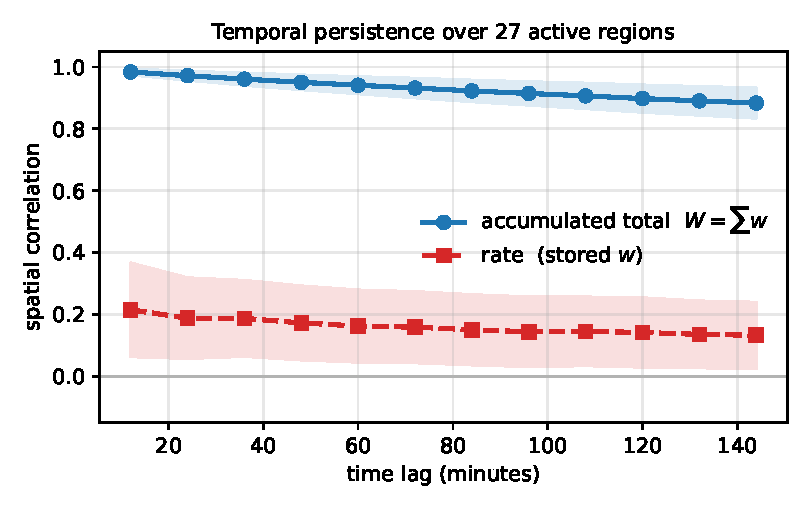
\includegraphics[width=0.66\textwidth]{figures/fig_autocorr.pdf}
\caption[Rate vs.\ total persistence]{\textbf{The rate is nearly unpredictable;
its integral is not.} Spatial correlation between winding frames separated by a
given time lag, averaged over the active-region corpus (shaded band: one standard
deviation across regions). The stored \emph{rate} decorrelates within minutes
(red), whereas the \emph{accumulated total} remains strongly correlated for hours
(blue). Forecasting the total is therefore tractable, but the skill it affords is
dominated by persistence---the theme of Chapter~\ref{ch:results}.}
\label{fig:autocorr}
\end{figure}

\paragraph{Spatial low-pass and downsampling.}
Before entering the network each frame is area-downsampled to a fixed width and
convolved with a separable Gaussian kernel. This is a deliberate, disclosed
choice: it discards fine spatial detail in favour of the large-scale envelope of
the field. The physical justification is that the small-scale content of the
winding field is effectively unpredictable, whereas its large-scale envelope
evolves coherently; removing the former lets the model concentrate its capacity
on the part of the field that can actually be forecast. The cost---loss of
sub-envelope structure---is real and is acknowledged wherever results are
reported. Figure~\ref{fig:pipeline} summarises the full pipeline from the raw
rate cube to the gap-aware training windows.

% Data pipeline: raw rate cube -> accumulated total -> normalized, low-passed windows.
\begin{figure}[!htbp]
\centering
\resizebox{\textwidth}{!}{%
\begin{tikzpicture}[
  font=\small, >=Latex, node distance=4mm,
  pstep/.style={draw, rounded corners=3pt, minimum height=13mm, text width=23mm,
               align=center, fill=black!4, inner sep=3pt},
  hl/.style={fill=green!12},
]
\node[pstep] (raw) {raw winding\\\texttt{wind}$[H,W,T]$};
\node[pstep, right=of raw] (sent) {drop sentinels\\\scriptsize$\mathrm{Time}\le 0$};
\node[pstep, right=of sent, hl] (cum) {accumulate\\$W[t]{=}\sum_{\tau\le t} w$\\\scriptsize(\emph{total}, persistent)};
\node[pstep, right=of cum] (asinh) {asinh$(\cdot/10^{3})$\\+ robust scale\\\scriptsize clip $[-1,1]$};
\node[pstep, right=of asinh] (low) {downsample\\+ Gaussian\\low-pass};
\node[pstep, right=of low, hl] (win) {gap-aware\\windows\\\scriptsize$t_{\text{in}}{=}10\!\to\!t_{\text{out}}{=}4$};
\foreach \a/\b in {raw/sent, sent/cum, cum/asinh, asinh/low, low/win}{\draw[->, thick] (\a) -- (\b);}
\end{tikzpicture}}
\caption[Data pipeline]{\textbf{Winding-flux data pipeline.} Missing frames
(sentinel timestamps) are removed, and the winding is accumulated over time into
the persistent \emph{total} winding $W[t]$ (Eq.~\ref{eq:cumsum}), the forecasting
target. The total is passed through
the sign-preserving asinh transform of Eq.~\eqref{eq:asinh} and a robust rescale,
spatially downsampled and low-passed (\S\ref{sec:data}), and finally cut into
gap-aware history/future windows for training (\S\ref{sec:training}).}
\label{fig:pipeline}
\end{figure}


\section{The Convolutional LSTM cell}
\label{sec:convlstm}

The temporal backbone of the model is the Convolutional LSTM (ConvLSTM) of
\citet{shi2015}, which adapts the Long Short-Term Memory unit of
\citet{hochreiter1997} to spatial data. A standard LSTM maintains a memory cell
gated by learned nonlinearities but treats its input as a flat vector, destroying
spatial structure. The ConvLSTM keeps the same gating logic but replaces every
matrix multiplication with a two-dimensional convolution, so that the hidden
state $h$ and cell state $c$ are \emph{feature maps} rather than vectors, and
spatial locality is preserved throughout the recurrence.

At each timestep the current input frame $x_t$ and the previous hidden state
$h_{t-1}$ (both feature maps) are concatenated along the channel axis and passed
through a single convolution whose output is split into four gate maps---input
$i$, forget $f$, candidate $g$ and output $o$:
\begin{align}
  i_t &= \sigma\!\big(W_i * [\,x_t, h_{t-1}\,] + b_i\big), &
  f_t &= \sigma\!\big(W_f * [\,x_t, h_{t-1}\,] + b_f\big), \nonumber\\
  g_t &= \tanh\!\big(W_g * [\,x_t, h_{t-1}\,] + b_g\big), &
  o_t &= \sigma\!\big(W_o * [\,x_t, h_{t-1}\,] + b_o\big),
  \label{eq:gates}
\end{align}
where $*$ denotes convolution and $\sigma$ the logistic sigmoid. The cell and
hidden states update as
\begin{equation}
  c_t = f_t \odot c_{t-1} + i_t \odot g_t,
  \qquad
  h_t = o_t \odot \tanh(c_t),
  \label{eq:cell}
\end{equation}
with $\odot$ the elementwise product. Computing all four gates with one
convolution is an efficiency choice; using ``same'' padding keeps the spatial
resolution fixed through the recurrence. Two implementation details matter for
stable training: the forget-gate bias $b_f$ is initialised to $+1$, so that the
cell defaults to \emph{remembering} its state early in training and gradients
propagate cleanly through time; and normalisation between stacked layers uses
group normalisation, which carries no running statistics and is therefore safe
to reuse across the unrolled decoding loop. Figure~\ref{fig:cell} traces the
internal dataflow of a single cell.

% ConvLSTM cell internals — one conv computes all four gates; cell/hidden update.
\begin{figure}[t]
\centering
\begin{tikzpicture}[
  font=\small,
  box/.style={draw, rounded corners=2pt, minimum height=7mm, minimum width=9mm, align=center},
  gate/.style={draw, circle, minimum size=6mm, inner sep=0pt},
  op/.style={draw, circle, minimum size=5.5mm, inner sep=0pt, fill=black!4},
  sig/.style={box, fill=blue!8},
  tnh/.style={box, fill=orange!12},
  >=Latex, node distance=6mm
]
% inputs
\node (xt)   at (0,-2.0) {$x_t$};
\node (hp)   at (0, 0.0) {$h_{t-1}$};
\node (cp)   at (0, 2.0) {$c_{t-1}$};
% concat + conv
\node[box, fill=black!5, minimum height=16mm] (cat) at (2.0,-1.0) {concat\\$[x_t,h_{t-1}]$};
\node[box, fill=green!10, minimum height=22mm, minimum width=13mm] (conv) at (4.2,-0.6)
      {Conv$2$D\\$\to 4C$\\channels};
\draw[->] (xt) -- (cat.south west|-xt);
\draw[->] (hp) -- (cat.north west|-hp);
\draw[->] (cat) -- (conv);
% four gate activations
\node[sig] (gi) at (6.6, 1.4) {$\sigma$};
\node[sig] (gf) at (6.6, 0.4) {$\sigma$};
\node[tnh] (gg) at (6.6,-0.6) {$\tanh$};
\node[sig] (go) at (6.6,-1.6) {$\sigma$};
\node[right=1mm of gi] {$i_t$};
\node[right=1mm of gf] {$f_t$};
\node[right=1mm of gg] {$g_t$};
\node[right=1mm of go] {$o_t$};
\foreach \g in {gi,gf,gg,go}{\draw[->] (conv.east) -- (\g.west);}
% cell-state line
\node[op] (mulf) at (9.2, 1.4) {$\odot$};
\node[op] (mulig) at (9.2,-0.1) {$\odot$};
\node[op] (add)  at (10.6, 1.4) {$+$};
\node[tnh, minimum width=7mm] (tc) at (12.0, 1.4) {$\tanh$};
\node[op] (mulo) at (12.0,-1.6) {$\odot$};
% c_{t-1} into f-mult
\draw[->] (cp) -- (cp-|mulf) node[midway,above,font=\scriptsize]{} -- (mulf.north);
\draw[->] (gf) -- (mulf);
\draw[->] (gi) to[out=0,in=180] (mulig.west);
\draw[->] (gg) to[out=0,in=180] ($(mulig.west)+(0,-0.0)$);
\draw[->] (mulf) -- (add);
\draw[->] (mulig) -- (mulig-|add) -- (add.south);
% c_t out
\node (ct) at (13.8, 1.4) {$c_t$};
\draw[->] (add) -- (ct);
\draw[->] (add) -- ++(0.0,0) -| (tc.north);
% h_t out
\draw[->] (tc) -- (tc|-mulo) -- (mulo.north);
\draw[->] (go) -- (mulo);
\node (ht) at (13.8,-1.6) {$h_t$};
\draw[->] (mulo) -- (ht);
\end{tikzpicture}
\caption[ConvLSTM cell]{\textbf{The Convolutional LSTM cell.} A single
$2$D convolution over the channel-concatenated input and previous hidden state
$[x_t,h_{t-1}]$ produces all four gate maps at once (input $i_t$, forget $f_t$,
candidate $g_t$, output $o_t$; Eq.~\ref{eq:gates}). The cell state updates as
$c_t=f_t\odot c_{t-1}+i_t\odot g_t$ and the hidden state as
$h_t=o_t\odot\tanh(c_t)$ (Eq.~\ref{eq:cell}). All states are feature maps, so
spatial structure is preserved through the recurrence.}
\label{fig:cell}
\end{figure}


\section{Encoder--forecaster model}
\label{sec:model}

The full model is an \emph{encoder--forecaster}: a stack of ConvLSTM layers first
reads the observed history, and a second stack then generates the future frames
autoregressively. Given an input clip of $T_{\text{in}}=10$ frames, the encoder
applies Eq.~\eqref{eq:gates}--\eqref{eq:cell} layer by layer and frame by frame,
accumulating the sequence into the hidden and cell states of every layer. No
output is produced during encoding; its sole purpose is to summarise the history
into the recurrent state.

Decoding then rolls the state forward for $T_{\text{out}}=4$ steps. At each step
the decoder stack advances the recurrent state and a $1\times1$ convolution maps
the top hidden map to a single-channel prediction. Crucially the model predicts a
\emph{residual}: the output is the previous frame plus a learned increment,
\begin{equation}
  \hat{x}_{t+1} = x_t + \Delta_\theta(h_t),
  \label{eq:residual}
\end{equation}
so that a do-nothing network falls back to \emph{persistence}---copying the last
frame---rather than collapsing to zero. This is the appropriate inductive bias
for a strongly persistent field and, as Chapter~\ref{ch:results} makes clear, it
also sets the correct baseline against which any genuine skill must be measured.
The predicted frame is fed back as the next decoder input, so errors compound
along the roll-out exactly as they would at deployment. Figure~\ref{fig:model}
shows the encoder, the state hand-off, and the autoregressive decoder together.

% Encoder--forecaster: encode 10 history frames, autoregressively decode 4 frames.
\begin{figure}[!htbp]
\centering
\begin{tikzpicture}[
  font=\small, >=Latex,
  frame/.style={draw, minimum size=6mm, fill=blue!7, rounded corners=1pt},
  pframe/.style={draw, minimum size=6mm, fill=orange!14, rounded corners=1pt},
  gframe/.style={draw, minimum size=6mm, fill=green!12, rounded corners=1pt},
  stack/.style={draw, rounded corners=3pt, minimum height=20mm, align=center, fill=black!4},
]
% ----- input history frames -----
\foreach \i/\x in {1/0,2/0.75,3/1.5}{\node[frame] (in\i) at (\x,3) {};}
\node at (2.25,3) {$\cdots$};
\foreach \i/\x in {9/3.0,10/3.75}{\node[frame] (in\i) at (\x,3) {};}
\node[font=\scriptsize] at (1.9,3.7) {input history\ \ $x_1,\dots,x_{10}$ ($t_{\text{in}}{=}10$)};
% ----- encoder -----
\node[stack, minimum width=34mm] (enc) at (1.9,1.2) {\textbf{Encoder}\\ConvLSTM $\times L$};
\foreach \i in {1,2,3,9,10}{\draw[->] (in\i) -- (in\i|-enc.north);}
% ----- state hand-off -----
\node[stack, minimum width=30mm, fill=black!7] (dec) at (7.4,1.2) {\textbf{Forecaster}\\ConvLSTM $\times L$};
\draw[->, very thick] (enc.east) -- node[above,font=\scriptsize]{state $(h,c)$} (dec.west);
% ----- decoded frames -----
\foreach \i/\x in {11/6.65,12/7.4,13/8.15,14/8.9}{\node[pframe] (out\i) at (\x,3) {};}
\node[gframe] (gt) at (9.9,3) {};
\node[font=\scriptsize] at (7.8,3.7) {forecasts\ \ $\hat{x}_{11},\dots,\hat{x}_{14}$ ($t_{\text{out}}{=}4$)};
\node[font=\scriptsize, green!45!black] at (9.9,3.7) {truth};
\foreach \i in {11,12,13,14}{\draw[->] (out\i|-dec.north) -- (out\i);}
% ----- residual + feedback -----
\node[draw, circle, minimum size=4.5mm, inner sep=0pt, fill=orange!8] (plus) at (7.4,-0.4) {$+$};
\node[font=\scriptsize, align=center] at (7.4,-1.15) {residual\\$\hat{x}_{t+1}=x_t+\Delta_\theta(h_t)$};
\draw[->] (dec.south) -- (plus);
\draw[->] (plus) -| (dec.south east) ;
% feedback loop: prediction becomes next input
\draw[->, orange!60!black] (out12.south) to[out=-90,in=90] ($(dec.north)+(0.9,0)$);
\node[font=\scriptsize, orange!55!black] at (8.9,1.95) {feed back};
% teacher forcing (train only)
\draw[->, dashed, green!45!black] (gt.south) to[out=-90,in=60] ($(dec.north east)+(-0.2,0)$);
\node[font=\scriptsize, green!45!black, align=center] at (10.7,1.2) {teacher\\forcing\\(train)};
\end{tikzpicture}
\caption[Encoder--forecaster]{\textbf{The encoder--forecaster model.} A stack of
$L$ ConvLSTM layers encodes the $t_{\text{in}}{=}10$ history frames into the
recurrent state $(h,c)$; a second stack then rolls the state forward for
$t_{\text{out}}{=}4$ steps. Each step predicts a \emph{residual}
$\hat{x}_{t+1}=x_t+\Delta_\theta(h_t)$ (Eq.~\ref{eq:residual}), so a null network
falls back to persistence, and feeds its own prediction back as the next input.
During training the fed-back frame may be replaced by the ground truth with
probability equal to the teacher-forcing ratio (dashed); at evaluation the model
runs purely autoregressively.}
\label{fig:model}
\end{figure}


During training the fed-back frame may instead be the ground-truth frame with a
tunable probability---\emph{teacher forcing}---which stabilises early optimisation
by anchoring the roll-out to real data; at evaluation teacher forcing is switched
off and the model runs purely on its own predictions.

\section{Training procedure}
\label{sec:training}

The model is optimised with Adam and a per-frame regression loss (a smoothed
$L_1$ / Huber criterion) between the predicted and true future frames, summed
over the $T_{\text{out}}$ horizon. Gradients are clipped in norm to curb the
occasional large update produced by rare high-amplitude frames, and the learning
rate follows a cosine decay across the training budget.

Evaluation follows a strict \emph{leave-one-active-region-out} protocol. Because
successive $12$-minute frames within a cube are highly autocorrelated, any split
that mixes frames from the same active region between training and test leaks
information and inflates the apparent score. The model is therefore trained on
the pooled windows of all active regions except one, and evaluated only on the
held-out region it has never seen. All figures and metrics in
Chapter~\ref{ch:results} are reported on such held-out regions, together with the
persistence baseline of Eq.~\eqref{eq:residual}, so that model skill is always
stated relative to the trivial forecast.
